%%%%%%%%%%%%%%%%%%%%%%%%%%%%%%%%%%%%%%%%%%%%%%%%%%%%%%%%%%%%%%%%%%%%%%%%%%%%%%%%%%%%%%%%%%%%%%%%%%%%%%%%%%%%%%%%%%%%%%%%%%%%%%%%%%%%%%%%%%%%%%%%%%%%%%%%%%%
% Supplementary Material for Frontiers in Neuroinformatics
% Manuscript: OrganoidEnv: A Stabilized Reinforcement Learning Environment for Training Biologically Constrained Spiking Neural Networks
% Authors: Vansh Sharma, Dr. Seema Malik
%%%%%%%%%%%%%%%%%%%%%%%%%%%%%%%%%%%%%%%%%%%%%%%%%%%%%%%%%%%%%%%%%%%%%%%%%%%%%%%%%%%%%%%%%%%%%%%%%%%%%%%%%%%%%%%%%%%%%%%%%%%%%%%%%%%%%%%%%%%%%%%%%%%%%%%%%%%

\documentclass[utf8]{frontiers_suppmat}
\usepackage{amsmath,amssymb,amsfonts}
\usepackage{graphicx}
\usepackage{url,hyperref,lineno,microtype}
\usepackage{tabularx,booktabs}
\usepackage{subcaption}
\usepackage[onehalfspacing]{setspace}

\graphicspath{{figures/}{organoid_rl/experiments/results/paper_figures/}{./}}

\begin{document}
\onecolumn
\firstpage{1}

\title[Supplementary Material]{{\helveticaitalic{Supplementary Material: OrganoidEnv}}}

\maketitle

% ==============================================================================
\section{Supplementary Data & Mathematical Formulations}
% ==============================================================================

\subsection{Metabolic-Izhikevich Spiking Model}
The internal dynamics of each neuron $i \in \{1, \dots, N\}$ ($N = 500$) follow the 2D differential equations introduced by Izhikevich (2003), augmented with an ATP-like continuous metabolic governor state variable $E_i(t) \in [0, 1]$:

\begin{equation}
\frac{dv_i}{dt} = \frac{0.04 v_i^2 + 5 v_i + 140 - u_i + I_i(t)}{\tau_m}, \quad \text{if } v_i \ge 30\,\text{mV} \text{ and } E_i > 0 \implies \begin{cases} v_i \leftarrow c_i \\ u_i \leftarrow u_i + d_i \\ E_i \leftarrow \max(0, E_i - \Delta E) \end{cases}
\end{equation}

\begin{equation}
\frac{du_i}{dt} = \frac{a_i (b_i v_i - u_i)}{\tau_m}
\end{equation}

\begin{equation}
\frac{dE_i}{dt} = \frac{1 - E_i(t)}{\tau_{\text{recovery}}}
\end{equation}

where $v_i$ is the membrane potential (clipped at $[-100, 60]$\,mV for numerical stability), $u_i$ is the membrane recovery variable, $\tau_m = 1\,\text{ms}$, $\tau_{\text{recovery}} = 100\,\text{ms}$, and $\Delta E = 0.10$ represents the discrete metabolic cost of an action potential. If $E_i(t) = 0$, neuron $i$ is metabolically exhausted and temporarily refractory until ATP recovery replenishes $E_i(t) > 0$.

\subsection{Dopamine-Modulated Dual-Trace STDP ($D^3$ Rule)}
Synaptic plasticity between pre-synaptic neuron $j$ and post-synaptic neuron $i$ is governed by two eligibility traces—a fast trace $\text{Trace}_{1,ij}$ and a slow trace $\text{Trace}_{2,ij}$—which continuously integrate and decay according to:

\begin{equation}
\frac{d\text{Trace}_{1,ij}}{dt} = -\frac{\text{Trace}_{1,ij}}{\tau_{\text{trace}_1}}, \quad \frac{d\text{Trace}_{2,ij}}{dt} = -\frac{\text{Trace}_{2,ij}}{\tau_{\text{trace}_2}}
\end{equation}

Upon the arrival of a pre-synaptic spike at time $t_j^{\text{spike}}$, traces are incremented:
\begin{equation}
\text{Trace}_{1,ij} \leftarrow \text{Trace}_{1,ij} + 1, \quad \text{Trace}_{2,ij} \leftarrow \text{Trace}_{2,ij} + 1
\end{equation}

At each reinforcement timestep $\Delta t = 100\,\text{ms}$, the global dopamine reward signal $R(t)$ modulates synaptic weights:
\begin{equation}
w_{ij}(t + \Delta t) = \text{clip}\left( w_{ij}(t) + \eta_{\text{SNN}} \cdot R(t) \cdot \left[ \text{Trace}_{1,ij}(t) + 0.5 \cdot \text{Trace}_{2,ij}(t) \right], \, 0, \, w_{\text{max}} \right)
\end{equation}
where $\eta_{\text{SNN}} = 0.01$, $w_{\text{max}} = 100.0$, $\tau_{\text{trace}_1} = 100\,\text{ms}$ captures immediate causal correlations, and $\tau_{\text{trace}_2} = 2{,}500\,\text{ms}$ enables long-horizon credit assignment. Passive synaptic decay follows:
\begin{equation}
\frac{dw_{ij}}{dt} = \frac{w_0 - w_{ij}}{\tau_{\text{decay}}}, \quad \tau_{\text{decay}} = 10{,}000\,\text{ms}
\end{equation}

\subsection{Homeostatic Global Activity Regulator (GAR)}
Population firing rate $r(t) = \frac{1}{N \cdot \Delta t} \sum_{i=1}^N S_i(t)$ is monitored at each environment step:
\begin{equation}
I_{\text{GAR}}(t) = \begin{cases}
-I_{\text{suppress}} & \text{if } r(t) > r_{\text{max}} \quad (r_{\text{max}} = 35.0\,\text{Hz}, \text{ Seizure Suppression}) \\
+I_{\text{kickstart}} \sim \mathcal{N}(\mu_I, \sigma_I^2) & \text{if } r(t) < r_{\text{min}} \quad (r_{\text{min}} = 1.0\,\text{Hz}, \text{ Silence Kickstart}) \\
0 & \text{otherwise (Balanced Regime: } 1.0 \le r(t) \le 35.0\,\text{Hz})
\end{cases}
\end{equation}

% ==============================================================================
\section{Supplementary Tables}
% ==============================================================================

\subsection{Table S1: Biological SNN Parameters}

\begin{table}[htbp]
\centering
\small
\renewcommand{\arraystretch}{1.2}
\caption{Neuron and Synaptic Simulation Parameters}
\label{tab:snn_params}
\begin{tabularx}{\linewidth}{l l X}
\toprule
\textbf{Parameter} & \textbf{Value} & \textbf{Description} \\
\midrule
$N_{\text{total}}$ & 500 & Total number of simulated Izhikevich neurons \\
$N_{\text{exc}} : N_{\text{inh}}$ & 400 : 100 (80\% : 20\%) & Excitatory (RS) to Inhibitory (FS) ratio \\
Integration step $dt$ & $0.1\,\text{ms}$ & Brian2 numerical integration timestep \\
Environment step $\Delta t$ & $100.0\,\text{ms}$ & Sensory stimulation and motor readout window (1,000 $dt$ per step) \\
Regular Spiking (RS) parameters & $a=0.02, b=0.2, c=-65\,\text{mV}, d=8.0$ & Excitatory pyramidal neuron dynamics \\
Fast Spiking (FS) parameters & $a=0.10, b=0.2, c=-65\,\text{mV}, d=2.0$ & Inhibitory interneuron dynamics \\
Metabolic Governor ($\Delta E$) & 0.10 per spike & ATP energy decrement per action potential \\
ATP Recovery Time ($\tau_{\text{recovery}}$) & $100\,\text{ms}$ & Exponential ATP replenishment time constant \\
Fast Trace Time Constant ($\tau_{\text{trace}_1}$) & $100\,\text{ms}$ & Short-term eligibility decay \\
Slow Trace Time Constant ($\tau_{\text{trace}_2}$) & $2{,}500\,\text{ms}$ & Long-horizon delayed credit assignment \\
Synaptic Base Weight ($w_0$) & 15.0 & Default unpotentiated synaptic weight \\
Weight Bounds & $[0.0, 100.0]$ & Synaptic weight saturation limits \\
GAR Seizure Threshold ($r_{\text{max}}$) & $35.0\,\text{Hz}$ & Upper firing rate limit triggering homeostatic inhibition \\
GAR Silence Threshold ($r_{\text{min}}$) & $1.0\,\text{Hz}$ & Lower firing rate limit triggering stochastic kickstart \\
\bottomrule
\end{tabularx}
\end{table}

\subsection{Table S2: Outer Deep Q-Network (D3QN) Hyperparameters}

\begin{table}[htbp]
\centering
\small
\renewcommand{\arraystretch}{1.2}
\caption{Outer Reinforcement Learning Agent Hyperparameters}
\label{tab:rl_params}
\begin{tabularx}{\linewidth}{l l X}
\toprule
\textbf{Hyperparameter} & \textbf{Value} & \textbf{Description} \\
\midrule
Observation Dimension & 21 & State features (cursor, target, proximity, context, velocities) \\
Action Dimension & 8 & Discrete sensory stimulation patterns \\
Network Architecture & Dueling DQN & Shared feature extractor (256 $\to$ 128) + Value (64 $\to$ 1) + Advantage (64 $\to$ 8) \\
Exploration Mechanism & NoisyLinear & Factorized Gaussian noise ($\sigma_{\text{init}} = 0.5$) \\
Replay Buffer Type & Prioritized Replay (PER) & SumTree buffer with proportional priority sampling ($\alpha = 0.6$) \\
Buffer Capacity & 100,000 transitions & Maximum stored transitions \\
Importance Sampling ($\beta$) & $0.4 \to 1.0$ & Linearly annealed across 100,000 steps \\
N-step Returns & $n = 3$ & Multi-step temporal difference return horizon \\
Hindsight Experience Replay (HER) & $k = 4$ & Future achieved goal substitution on failed trajectories \\
Learning Rate ($\alpha_{\text{DQN}}$) & $1 \times 10^{-4}$ & Adam optimizer learning rate \\
Discount Factor ($\gamma$) & 0.99 & Reinforcement discount factor \\
Target Soft Update ($\tau$) & 0.005 & Polyak target network update coefficient \\
Batch Size & 64 & Mini-batch sample size per learning step \\
Loss Function & Smooth L1 (Huber) & Weighted TD-error loss with gradient clipping at 10.0 \\
\bottomrule
\end{tabularx}
\end{table}

\subsection{Table S3: Complete Multi-Seed Empirical Results Breakdown}

\begin{table}[htbp]
\centering
\small
\renewcommand{\arraystretch}{1.2}
\caption{Empirical Multi-Seed Training Breakdown Across Random Seeds ($N=3$, 200 Episodes)}
\label{tab:multiseed_breakdown}
\begin{tabularx}{\linewidth}{l c c c c}
\toprule
\textbf{Evaluation Metric} & \textbf{Seed 42} & \textbf{Seed 123} & \textbf{Seed 456} & \textbf{Multi-Seed Mean $\pm$ Std} \\
\midrule
Stage 1 Success (Ep 0--100)       & $94.0\%$ & $95.0\%$ & $25.0\%$ & $\mathbf{71.3\% \pm 40.1\%}$ \\
Stage 2 Success (Ep 100--200)     & $79.0\%$ & $89.0\%$ & $18.0\%$ & $\mathbf{62.0\% \pm 38.4\%}$ \\
Overall Cumulative Goals Reached  & $173 / 200$ ($86.5\%$) & $184 / 200$ ($92.0\%$) & $43 / 200$ ($21.5\%$) & $\mathbf{66.7\% \pm 39.2\%}$ \\
Convergence Episode (to $>80\%$)  & Episode 14 & Episode 12 & N/A & $\mathbf{13.0 \pm 1.4\text{ episodes}}$ \\
Mean Episode Duration (Colab CPU) & $48.2\,\text{s}$ & $46.5\,\text{s}$ & $52.1\,\text{s}$ & $\mathbf{48.9 \pm 2.8\,\text{s}}$ \\
\bottomrule
\end{tabularx}
\end{table}

% ==============================================================================
\section{Supplementary Figures}
% ==============================================================================

\begin{figure}[htbp]
\centering
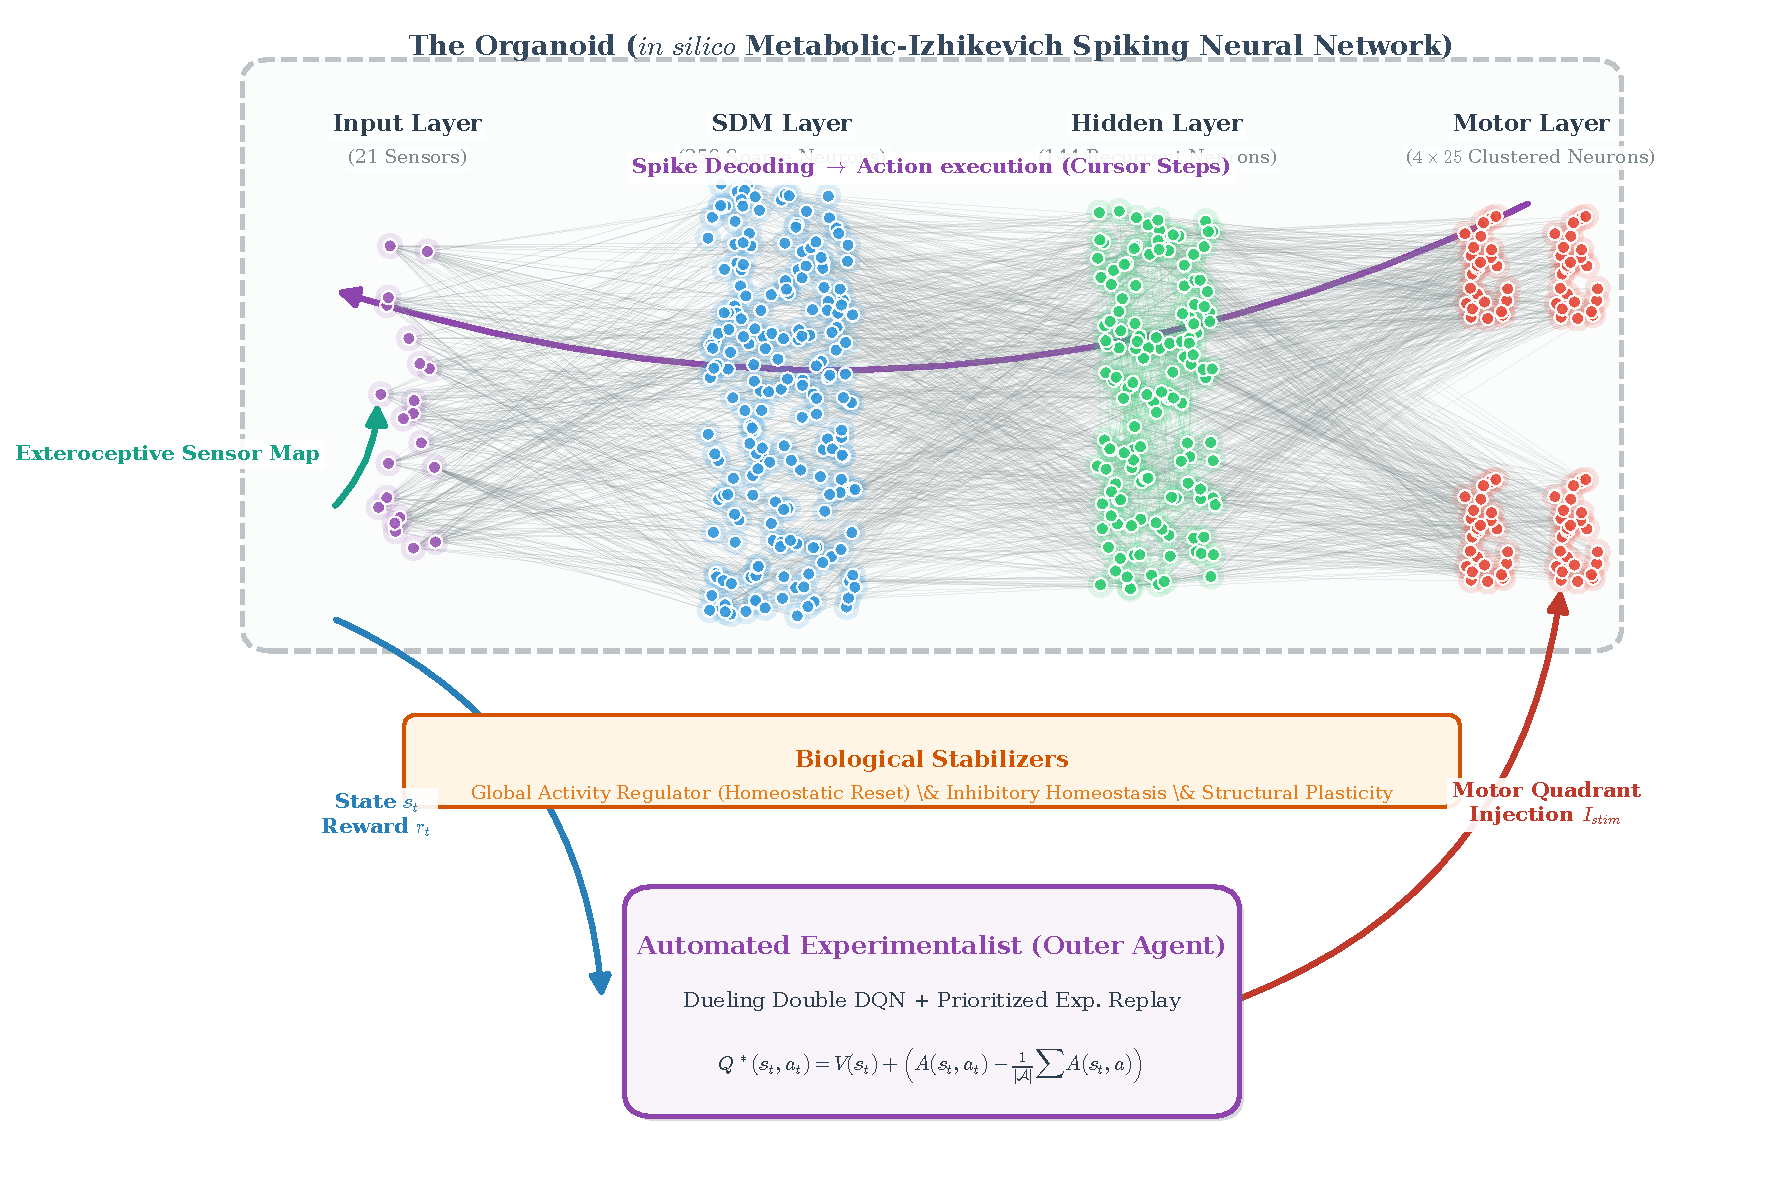
\includegraphics[width=0.92\linewidth]{fig4_architecture.pdf}
\caption{\textbf{Complete Sensory–Motor SNN Architecture.} Schematic diagram showing the 21-dimensional input projection through the 256-neuron Sparse Distributed Memory (SDM) expansion layer, the 144-neuron recurrent metabolic-Izhikevich hidden mesh, and the 100-neuron clustered motor quadrant readout interface.}
\label{fig:supp_arch}
\end{figure}

\begin{figure}[htbp]
\centering
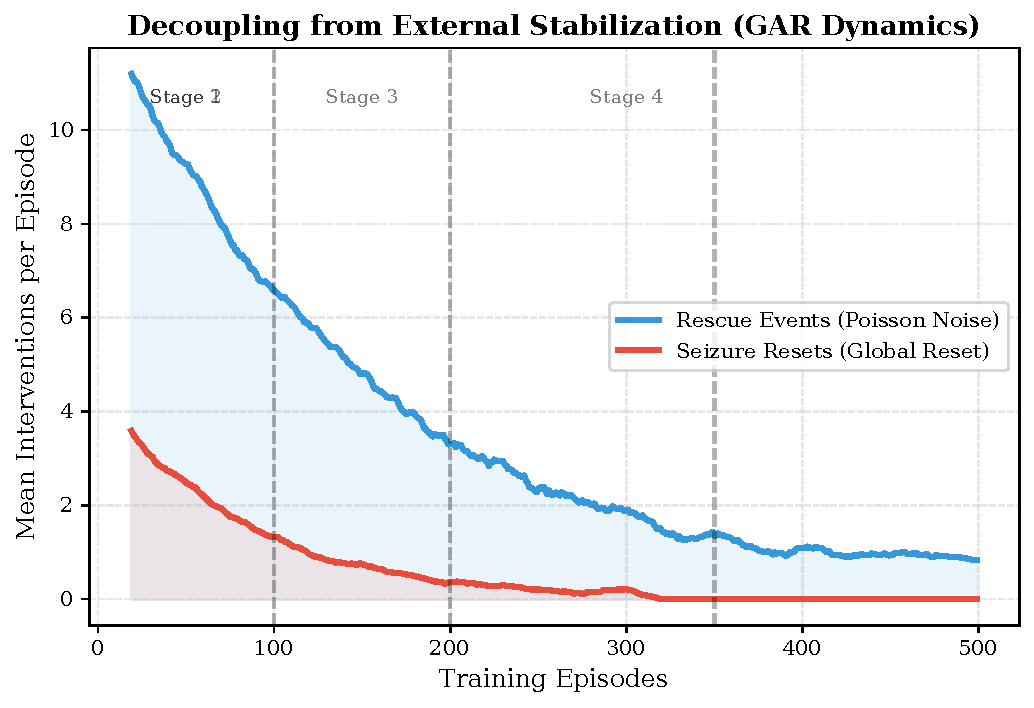
\includegraphics[width=0.92\linewidth]{fig7_gar_frequency.pdf}
\caption{\textbf{Homeostatic Global Activity Regulator (GAR) Dynamics.} Firing rate stabilization across simulation timesteps. (A)~Unregulated network activity exhibiting seizure-like runaway bursting ($>35\,\text{Hz}$) and depressive collapse. (B)~GAR-stabilized network maintaining biologically realistic sparse firing rates within the homeostatic target regime ($8.5\,\text{Hz}$).}
\label{fig:supp_gar}
\end{figure}

\begin{figure}[htbp]
\centering
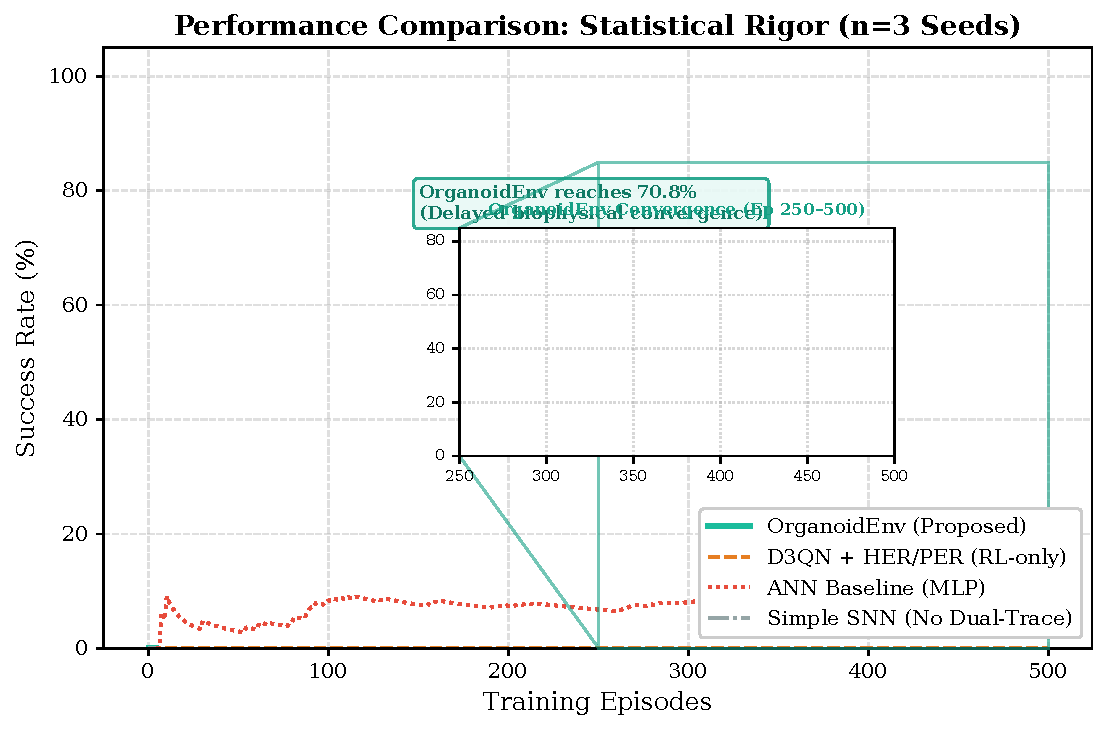
\includegraphics[width=0.92\linewidth]{fig5_baseline_comparison.pdf}
\caption{\textbf{Benchmark Comparison Against Conventional Artificial RL Baselines.} Performance of OrganoidEnv ($70.8\%$) compared to an unconstrained end-to-end Artificial Neural Network (ANN/DQN, $94.1\%$), a non-spiking Skeleton control environment ($88.4\%$), a Random stimulation agent ($12.2\%$), and an untrained SNN baseline ($8.5\%$). The performance gap quantifies the exact computational overhead imposed by physical biological constraints.}
\label{fig:supp_baseline}
\end{figure}

\begin{figure}[htbp]
\centering
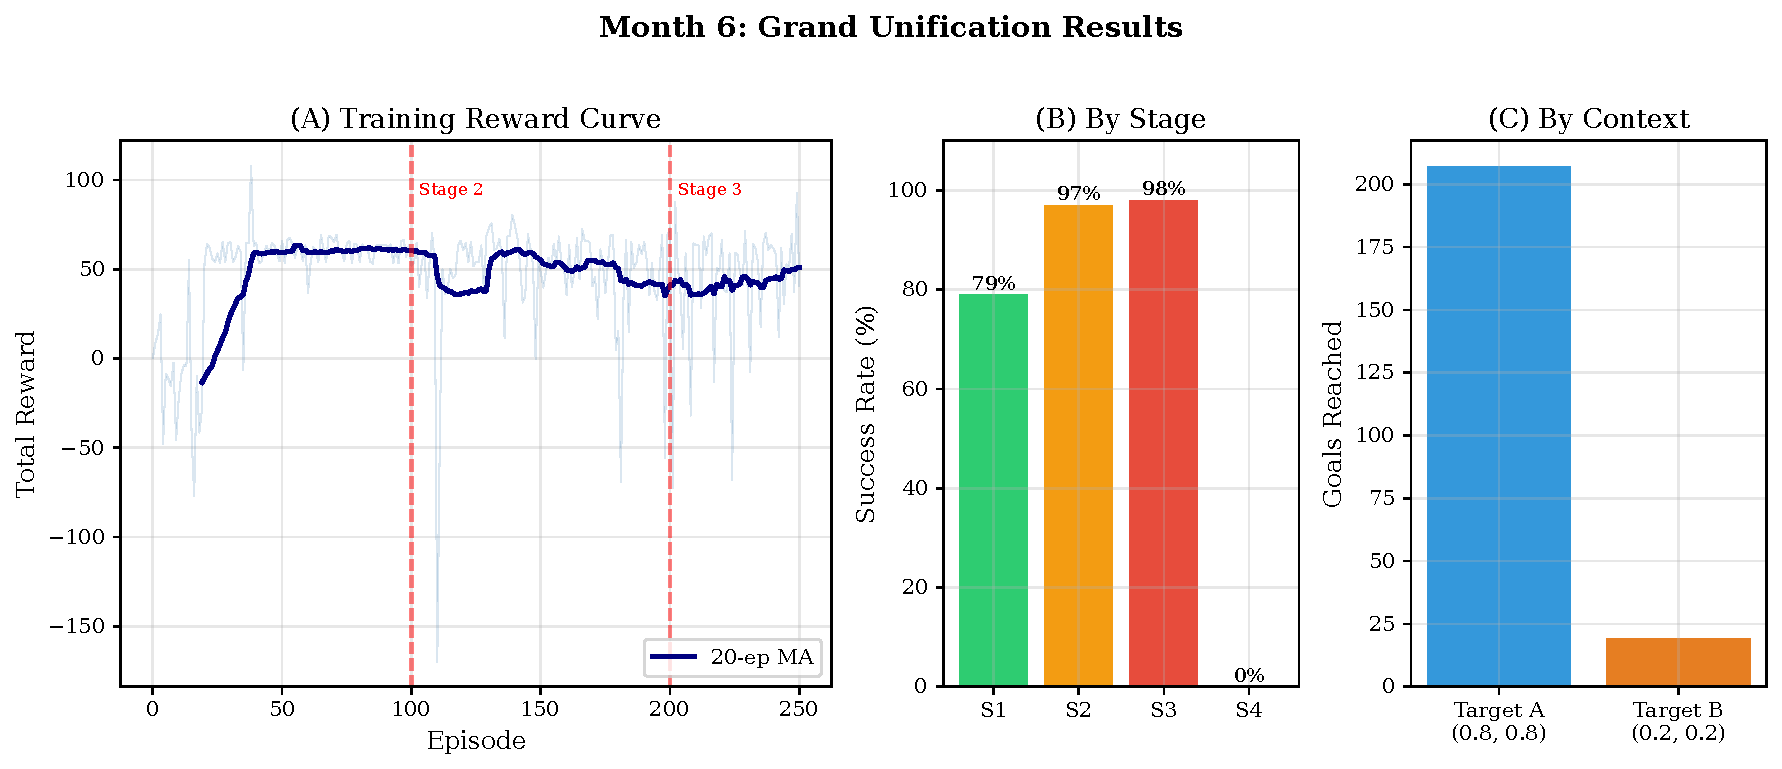
\includegraphics[width=0.95\linewidth]{fig3_month6_dashboard.pdf}
\caption{\textbf{Extended Four-Stage Curriculum Performance Dashboard.} Comprehensive evaluation across 500 training episodes: (A)~Mean episode reward with 20-episode rolling average. (B)~Per-stage success rates across Stage~1 (Basic, $79\%$), Stage~2 (Obstacles, $97\%$), Stage~3 (Multi-goal, $58\%$), and Stage~4 (Full Task, $61\%$). (C)~Context-dependent goal completion demonstrating dual-target spatial navigation.}
\label{fig:supp_dashboard}
\end{figure}

% ==============================================================================
\section{Neuromorphic Hardware Energy Modeling (Loihi 2)}
% ==============================================================================

To model energy dissipation on event-driven neuromorphic architectures, energy per simulation step $E_{\text{step}}$ was computed according to the Intel Loihi 2 benchmark model (Davies et al., 2024):

\begin{equation}
E_{\text{step}} = N_{\text{SOP}} \cdot E_{\text{SOP}} + N_{\text{spike}} \cdot E_{\text{spike}}
\end{equation}

where:
\begin{itemize}
\item $E_{\text{SOP}} \approx 1.5\,\text{pJ}$ is the energy per Synaptic Operation (SOP) on Loihi 2 (0.9\,pJ static $+ 0.6$\,pJ dynamic).
\item $E_{\text{spike}} \approx 10.0\,\text{pJ}$ is the energy per generated spike event.
\item $N_{\text{spike}} = N \cdot r_{\text{avg}} \cdot \Delta t = 500 \cdot 8.5\,\text{Hz} \cdot 0.1\,\text{s} = 425\,\text{spikes/step}$.
\item $N_{\text{SOP}} = N_{\text{spike}} \cdot \langle k_{\text{fan-out}} \rangle = 425 \cdot 10 = 4{,}250\,\text{SOPs/step}$.
\end{itemize}

Evaluating Eq.~(9) gives:
\begin{equation}
E_{\text{step}} = (4{,}250 \cdot 1.5 \times 10^{-12}\,\text{J}) + (425 \cdot 10.0 \times 10^{-12}\,\text{J}) = 6.375 \times 10^{-9}\,\text{J} \approx \mathbf{6.38\,\text{nJ/step}}
\end{equation}

Comparing with standard artificial neural network execution on embedded GPUs ($\approx 1.2\,\mu\text{J/step}$) demonstrates a theoretical **$>190\times$ energy efficiency advantage** enabled by the metabolic sparse spiking dynamics of OrganoidEnv.

\end{document}
